\chapter{Video Indexing: From signal processing to knowledge reasoning}
\label{state2}

Since multimedia resources are playing an increasingly outstanding role in our lives, the previous two decades have marked a great move 
of research for semantic analysis of multimedia contents in order to enable computational interpretation and processing of 
such resources. In fact, video analysis and retrieval topic have attracted considerable interest from both industry and academia, 
in which the key technology copes with data overload problem. The overriding interest of this topic is to model, represent and 
organize the large multimedia data for further efficient use and accessibility. The main aim can be stated as to provide 
pertinent multimedia contents that are relevant to a user inquiry \citep{Jaimes2005,Lew2006,Feng2013}.

The main focus of this chapter is to explore the research achievements in multimedia information retrieval and 
indexing, mainly in the enhancement of large-scale video content analysis and indexing 
\citep{Dasiopoulou2005, Snoek2008, Gani2015}. Thus, the present chapter sheds light on actual trends 
and opportunities to enhance multimedia content indexing efficiency through the use of ontology based approaches. 

	
\section{From low-level to knowledge based indexing}

	Ontologies, as knowledge database, have been emerged from an 
	interesting conceptualization paradigm to a very promising modeling technology for multimedia 
	retrieval. Ontologies enable meaning driven retrieval process through a machine-understandable 
	form of a content description.

	Earlier research in multimedia feature extraction focused mainly on the visual modality and involved frame-based 
	and object-based approaches \citep{Puri2000,Deb2004,Snoek2005}. Frame-based approaches deal with low-level features
	(such as histograms, colors, textures, motion, \dots{}) in order to detect a shot or to query by example 
	\citep{Brunelli1999,Antani2002,Kang2003,Smith2003}. These approaches became standard procedures and were 
	easy to compute, however,  they were not suitable to detect fine-grained semantics in a multimedia resource. 
	Thus, frame-based features were not able to get detailed semantic interpretation, but basically macro-grained 
	(particularly for detecting the subject of a multimedia resource like sports, news, \dots{}).
	Object-based approaches were proposed in order to overcome low-level based features limits for the description 
	of a multimedia content and to fill the gap between  perceptual properties and semantic meaning of a multimedia content. 
	In fact, object-based approaches deal with low-level features for an individual region instead of the whole content.
	This means that object-based approaches are suitable to detect high-level features like \emph{``table''}, 
	\emph{``chair''}, \emph{``car''}, \emph{``person''}, \dots{} \citep{Snoek2006,Lew2006,Spyrou2008}. 
	Many models have been proposed to identify semantic concepts in images \citep{Jurie2005,Yang2007,Wang2010} 
	and audio \citep{You2010,Feki2011,Rawat2013}. However, all these models raised one fundamental \revAnglais{question:} 
	\emph{Which semantic concepts should these models focus on and deal with?}
	
	In order to promote researches on multimedia analysis and to deliver a common set of semantic concepts, 
	the \textit{Moving Pictures Expert Group} (MPEG) have proposed the MPEG-7 \citep{Salembier2002} standard 
	for describing a multimedia content. The aim of MPEG-7 is to address a wide variety of media types and 
	to describe audiovisual information through providing a rich set of standardized tools that generate 
	and understand audiovisual features. Hence, the MPEG-7 standard defined more than $140$ semantic concepts
	that can describe  a multimedia \revAnglais{content. However,} as thoroughly elaborated in \citep{Naphade2006}, 
	some  practical obstacles have hindered the emerging research works and efforts in the multimedia content 
	analysis field, and the MPEG-7 received a weak attention from multimedia research community. 
	Firstly, many semantic concepts defined in MPEG-7 were not suitable for an automated detection. 
	For an example, it was very hard to multimedia content analyzers to  discover a semantic concept like 
	\emph{``remarkable people''} (defined in MPEG-7). Secondly, most of multimedia retrieval approaches were 
	based on statistical machine-learning techniques \citep{Deb2004}. These \revAnglais{latters} use annotated datasets to 
	build models and classifiers. However, datasets (and particularly training ones) were insufficient and 
	\revAnglais{non-standardized} to promote researches on multimedia semantics.
	
	To address these two issues, and to supply \revAnglais{large annotated multimedia datasets} that support a common set 
	of semantic concepts, the \textsc{LsCom} ontology (for \textit{Large Scale Concept Ontology for Multimedia}) 
	was proposed \citep{Kennedy2006,Naphade2006}. At first, a set of $1~000$ semantic concepts were defined and 80 
	hours of broadcast news video were manually annotated aiming at providing a valuable resource for the multimedia 
	research community. Actually, \textsc{LsCom} provides more than $2~500$ concepts. Many concept detection researches 
	began to be used successfully by exploring the  \textsc{LsCom} ontology: \textit{VIREO-374} \citep{Jiang2007, Jiang2010} 
	and \textit{Columbia374} \citep{Yanagawa2007} are able to detect up to $374$ semantic concepts in a visual content, 
	and \textit{Mediamill101} \citep{Snoek2006} is able to detect up to 101 semantic concepts. \textsc{LsCom} is 
	used also as a basis of many video annotation tools \citep{Garnaud2006,Worring2006,Ksentini2012}.
	
	Evaluation campaigns have played a significant role for the progress in semantic concept detection within a multimedia 
	content; The evaluation campaign \textsc{TrecVid} \citep{Smeaton2009, Over2013} has played the most significant
	role \citep{Snoek2010} by exploring the \textsc{LsCom} ontology resources. \textsc{TrecVid} intends to benchmark 
	search engines and to promote the content-based retrieval via open metrics-based evaluation. 
	As outlined in \citep{Snoek2010,Over2013}, experiments in \textsc{TrecVid} have led to conclude that available 
	semantic concept detection approaches \revAnglais{cannot} be generalized to any semantic concept. Indeed, these approaches 
	focus on identifying  objects in a content without dealing with implicit information: concepts co-occurrence and 
	the context in which an object is defined \citep{Feng2012,Feng2016}.
	
	\begin{description}
		\item[\textit{\textbf{Concepts co-occurrence}}] Earlier object detection approaches considered that a 
		detector is modeled for a single semantic concept. It also means that for detecting a set of semantic 
		concepts in a content, a set of detectors are simultaneously taken into consideration. Nevertheless, 
		a semantic relationship between this set of concepts could be explored. 
		Thus, authors in  \citep{Naphide2001} displayed a probabilistic model to explore inter-concept 
		relationships. Many other works \citep{Feng2012, Zheng2013} (to cite a few) followed 
		this promising track by computing similarities between detected concepts from an annotated multimedia 
		dataset (a training dataset). As an example, when the semantic concepts \emph{``sand''} and \emph{``sky''} 
		are detected in a content with a certain probability, a chance to consider that the concept \emph{``desert''} 
		is present should be increased (even if this concept was not detected), and a chance to consider that the 
		concept \emph{``Penguin''} is present should be decreased. Therefore, the co-occurrence of concepts is taken 
		a serious consideration in multimedia retrieval community.

		\item[\textit{\textbf{Contexts}}] In general, a multimedia content interpretation is an outcome of a defined 
		context in which contained semantic objects are defined \citep{Dumitrescu2009}. Therefore, the \emph{``context''} 
		emerged as a great opportunity to contribute to multimedia analysis enhancement 
		\citep{Elgesem2007,Jiang2009,Hori2003,Fauzi2014,Zhang2014,Schoeffmann2015}. 
		Many context-based multimedia retrieval systems used the context approach with an informal definition 
		\citep{Cioara2009, Nguyen2010, Parsons2009,PerpetualCoutinho2012,Hamadi2014}: In fact, contexts are defined 
		manually by authors. Consequently, these approaches are based on manual list of contexts to consider and 
		a set of semantic concepts that are defined under each context.
	\end{description}

	In summary, context based approaches and semantic co-occurrence exploration are capturing the attention of the 
	multimedia retrieval community and are being considered as promising research trend toward better semantic 
	interpretation capabilities for multimedia contents. 
	\revAnglais{Yet, these new approaches are moving increasingly toward availing knowledge management capabilities 
	(like ontology) in order to handle concepts, contexts and their relationships.}
	
\section{Semantic Multimedia Indexing: Towards Knowledge-Based Approaches}

	In this section, we exhibit an overview on some research works that targeted to explore
	knowledge databases in order to enhance the multimedia analysis accuracy. We display 
	how these databases are modeled, then we discuss their expressiveness levels, and after 
	enumerating related works, we talk over our motivation to propose a knowledge-based approach 
	in order to enhance semantic interpretations.

	\subsection{Ontology Modeling}
	
	Many research works expose different models for developing 
	and managing ontologies \citep{Sure1999,Fernandez-Lopez1999,Noy2001,Vrandecic2005,Gargouri2010,Terkaj2014,Zablith2015}.
	Commonly, ontology modeling consists in 
	defining some steps in order to represent the main tasks to build ontologies starting from an existing knowledge 
	source. The most important steps are: (1) the ontology structure, (2) the ontology population, (3) the reasoning 
	process, and (4) the ontology evolution.
		
		\begin{description}
			\item[\textbf{\textit{Ontology structure}}]
			The ontology structure is the process of knowledge organization 
			by defining concepts and their expected relationships. 
			\emph{OWL} (\emph{Web Ontology Language}) is a standard used for
			modeling and exchanging ontologies and is designed to support the \emph{Semantic Web} 
			\citep{Staab2009}. Semantically, \emph{OWL} is based on \emph{Description Logics} 
			(\emph{DL}) \citep{Baader2003}. \emph{OWL} ontologies are categorized into three types
			depending on their expressive level: from \emph{OWL-Lite} to \emph{OWL-DL}.
			%,to finally \emph{OWL-Full}.
			These two expressive levels differ in their 
			complexity and may be used depending on required inference simplicity or 
			formality of descriptions.

			\item[\textbf{\textit{Ontology Population}}]
			Ontology Population is the process of knowledge acquisition by analyzing and 
			transforming unstructured, 
			semi-structured and/or structured source data into ontology instances. 
			This process looks for identifying instances of concepts and interrelationships 
			of an ontology. Manual population by a domain expert is a costly and time consuming 
			task, then, automatic/semi-automatic approaches are considered 
			\citep{Song2009, Faria2011}.
	
			\item[\textbf{\textit{Inference and Rules}}] Rules are of the form of an implication between 
			an antecedent (\emph{body}) and consequent (\emph{head}). So, when combining 
			ontologies and rules for domain conceptualization and inference modeling, 
			ontologies can enhance and enrich the amount of knowledge that it can represent.

			\item[\textbf{\textit{Ontology Evolution}}]
			The ontology content has to evolve continuously throughout its 
			life cycle in order to be able to answer different change requirements. 
			The Ontology evolution seeks to grow the background knowledge in order to 
			better enrich its semantic capabilities. This evolution process consists 
			in updating and validating concepts and semantic relationships
			\citep{Gargouri2010, Paliouras2011b, Petasis2011}.
			Current ontology evolution works 
			give more attention to the way to enrich the ontology content: 
			from fully automatic to fully manual.
			Typically, a content validation by a domain expert  is considered as the most
			common process to ensure a valuable ontology content.
		\end{description}

		Ontologies are powerful tools to specify concepts and their interrelationships. 
		Several research areas have focused on ontologies for knowledge management.
		More particularly, information retrieval systems use ontologies 
		in order to enhance a machine ability to understand  the
		document semantic contents. Nevertheless, the very specific nature of these systems requires to handle 
		ontologies with specific considerations.

	\subsection{Ontology Expressiveness}
		As discussed above, ontologies could have a varying degrees of 
		expressiveness: \emph{OWL-Lite} and \emph{OWL-DL}. We discuss in the 
		following these two levels of expressiveness:

		\subsubsection{Light Ontologies:} are modeled as direct graphs in which nodes 
		represent semantic concepts. The relationships between these nodes depict links that 
		associate corresponding concepts and that express semantic nearness \citep{Reimer2012}. 

		These ontologies were used under a varying shapes in order to improve multimedia 
		retrieval and indexing. For instance, concept hierarchies \citep{Naphade2006,Deng2009}, 
		visual taxonomies \citep{Fei-Fei2005,Griffin2008a,Yao2010}, and semantic hierarchies 
		\citep{Fan2008,Li2010} have been used for visual content annotation.

		Light ontologies have been used to narrow the semantic gap. In fact, many works 
		have reported an improvement in visual multimedia (image) indexing and annotation 
		accuracy \citep{Tousch2008, Yao2010,Martinet2011}. Nevertheless, light ontology 
		based approaches are just used to model explicit knowledge without exploring implicit 
		one: it is leading importance to explore the inter-concepts correlation (explicit knowledge) 
		in order to discover and deduce newer (implicit) knowledge \citep{Bannour2011,Dingli2011}. 
		In fact, these approaches have used \revAnglais{neither} the expressiveness \revAnglais{nor} the reasoning 
		capabilities provided by ontologies.

			
		\subsubsection{Formal Ontologies}

		The description language (DL) \citep{Baader2003} are a formal knowledge representation formalisms
		that are used to model the terminological knowledge of application domain in a structured manner.
		DL have been used in various application domains, but their most noted success is the adoption 
		of the DL-based language OWL \citep{Horrocks2003} as the standard ontology language for the 
		semantic web \citep{Berners-Lee2001}.

		\begin{figure}[ht]
			\centering
			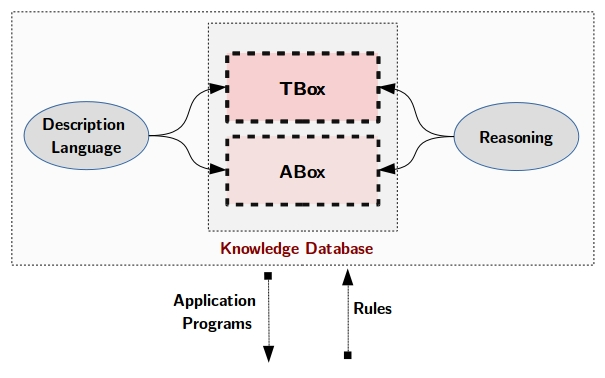
\includegraphics[scale=0.7]{figures/state_fig6}
			\caption{A knowledge Representation System Architecture of a knowledge
				representation system based on Description \citep{Baader2003}}
			\label{state_fig6}
		\end{figure}

		Description Language-based knowledge base $\mathcal{K}$(or an ontology) can be defined as 
		a pair $\mathcal{K} = (\mathcal{T}, \mathcal{A})$  where $\mathcal{T}$ (called the \emph{TBox}), 
		is a set of \textit{concept axioms} and \textit{role axioms}, and $\mathcal{A}$ (called the 
		\emph{ABox}), is a set of \textit{assertional axioms} (see figure \ref{state_fig6}).

		The \emph{concept axiom} has the form $C \sqsubseteq D$ where $C$ and $D$ are concept expressions.
		The \emph{role axiom} \revAnglais{has} the form $R \sqsubseteq S$ where $R$  and $S$ are role expressions. 
		Finally, the \emph{Assertional axioms} have the form $C(a)$ where $C$ is a concept and $a$ 
		is an individual name, or that have the form $R(a,b)$, where $R$ is a role and $a$ and $b$ 
		are individual names.

		In the Description Language, an interpretation $I$ is defined as follows: $I=\mathcal{I} 
		= \langle{}\triangle^{\mathcal{I}}= , \cdot^{\mathcal{I}}\rangle{}$ that consists of
		a non-empty set $\triangle^{\mathcal{I}}$ and an interpretation function $\cdot^{\mathcal{I}}$, 
		which maps from individuals, concepts and roles to elements of the domain, subsets of the domain 
		and binary relations on the domain, respectively.

		For a given interpretation $\mathcal{I} $, we can say that $\mathcal{I} $ satisfies a concept 
		axiom $C \sqsubseteq D$  (respectively $R \sqsubseteq S$) if $C^{\mathcal{I}} \subseteq 
		D^{\mathcal{I}} $ (respectively $R^{\mathcal{I}} \subseteq S^{\mathcal{I}}$). Moreover, 
		$\mathcal{I}$ satisfies a concept assertion $C(a)$ (respectively $R(a,b)$) if 
		$a^{\mathcal{I}} \in C^{\mathcal{I}}$ (respectively $(a^{\mathcal{I}},b^{\mathcal{I}}) 
		\in R^{\mathcal{I}}$).

		An interpretation $\mathcal{I}$ is called a model of an ontology $\mathcal{K}$ if and only 
		if it satisfies each axiom in $\mathcal{K}$. A concept name $C$ in an ontology $\mathcal{K}$, 
		is unsatisfiable if for each model $\mathcal{I}$ of $\mathcal{K}$, $C^{\mathcal{I}} = \varnothing$. 
		An ontology $\mathcal{K}$ is incoherent if there exists an unsatisfiable concept name in $\mathcal{K}$. 
		An ontology $\mathcal{K}$ is inconsistent if and only if it has no model.

		DL languages are identified with the concept constructors that they allow. For instance, the minimal 
		propositionally closed language allowing for the constructors $\sqcap$ ( conjunction), $\sqcup$ 
		(disjunction), $\neg$ (negation), $\forall$ (value restriction) and $\exists$ (existential restriction)
		is called $\mathcal{ALC}$. In \citep{Baader2003}, the author enumerates all the constructors used to 
		identify various Description Logic formalisms ($\mathcal{N}$, $\mathcal{Q}$, $\mathcal{O}$,
		$\mathcal{F}$, $\mathcal{U}$, \dots{}).

		Once a description of application domain using DL, the latter can make inference through 
		deducing implicit consequences from the explicitly represented knowledge. The subsumption is 
		the basis inference on concept descriptions: given two concept descriptions $C$ and $D$, 
		the subsumption problem $C \sqsubseteq D$ is the problem of checking whether the concept description 
		$D$ is more general \revAnglais{than} the concept description $C$. Then, the subsumption problem tries to determine whether 
		the first concept denotes in every interpretation a subset of the set denoted by the second one. $C$ 
		is subsumed by $D$, with respect to a \emph{TBox} $\mathcal{T}$, if in every model of $\mathcal{T}$, 
		$D$ is more general than $C$, i.e., the interpretation of $C$ is a subset of the interpretation of 
		$D$. This can be denoted as $C \sqsubseteq_{\mathcal{T}} D$.

		Description language based ontologies have been successfully used to achieve some interesting
		reasoning capabilities in the context of semantic multimedia analysis. In fact, such an ontology 
		formalism enables an intensive use of inference rules on the managed knowledge to perform advanced 
		multimedia semantic analysis, attaining thus a semantic interpretation that a human perception and 
		cognition can deliver. In order to achieve such an inference tasks, the description language \revAnglais{is} 
		based on a set of concepts and relationships between them. The lattes are called roles 
		(denoted with $\mathcal{R}$). Axioms are used to capture the conditions that need to be met 
		by consistent and coherent interpretations (the states of the domain). Therefore, the knowledge 
		management tasks within an ontology could be formalized as:

		\begin{itemize}
			\item \textbf{\textit{Deduction:}} is a task where the interpretation is an instantiation of 
			formal knowledge consistent with evidence about the real-world domain 
			\citep{Hartz2007,Hudelot2008,Dasiopoulou2009a}.
			
			\item \textbf{\textit{Abduction:}} is a task where the interpretation is an instantiation of 
			formal knowledge which allows to deduce the evidence \citep{Shanahan2005,Peraldi2007,Atif2014}.
		\end{itemize}
		The deduction and the abduction reasoning tasks were introduced as inference standards. 
		For the deduction reasoning, if $\sum$ is a logical theory and $\alpha$ a set of facts, 
		through deduction is verified whether $\varphi$ is logically entailed, that is whether $\sum, 
		\alpha \models \varphi$. For the abduction reasoning, given $\sum$ and $\varphi$, the abduction 
		consists in looking for an \emph{explanation} $\alpha$ so that the entailment $\sum, \alpha \models 
		\varphi$ is true.

		In \citep{Neumann2008,Moeller2008,Dasiopoulou2010,Bannour2014}, a comprehensive survey on 
		the use of formal (description language based) ontologies for multimedia semantic analysis
		is exposed. In the following section, we enumerate some of these works.

		



		\subsection{Related Work on Knowledge-Based Approaches for Multimedia Analysis}

		In the last fifteen years, ontologies have been emerged from an interesting conceptualization paradigm 
		to a very promising modeling technology for multimedia retrieval. Ontologies enable meaning driven 
		retrieval process through a machine-understandable form of a content description. 
		In the following, we enumerate some multimedia ontologies outlining main characteristics.

		The \emph{Harmony} ontology \citep{Hunter2001}, the \emph{aceMedia} ontology 
		\citep{ Petridis2004} and the	\emph{Rhizomik} \citep{Garcia2005} ontology are first initiatives 
		to attach formal semantic to MPEG-7.  These ontologies have been explored to support 
		semantic image /video analysis and annotation, addressing many content domains, including 
		pancreatic cell images (for \emph{Hamony}),  soccer video (for \emph{Rhizomik}), \dots.  
		More recent MPEG-7 based ontologies, like \emph{SmartWeb} \citep{Oberle2007}, \emph{DS-MIRF} 
		\citep{Tsinaraki2007}, \emph{COMM} \citep{Arndt2007} and \emph{Boemie} \citep{Dasiopoulou2009}, 
		focused on a fully translation/mapping of the complete MPEG-7 specification into \emph{OWL}. 
		
		These ontologies were mostly used in analyzing and annotating sport oriented multimedia contents.
		In their majority, enumerated ontologies have been constructed manually, and their knowledge structures 
		are rather focused on low-level and high-level features (as classes), and their spatial-temporal 
		relationships for particular content domains. Thus, these approaches are limited to provide a 
		formalism that \revAnglais{allows} to use ontologies as repositories for storing knowledge. So, there is no
		correspondence between the expressive power provided by the adopted representation language, and 
		the constructed ontology definitions. Hence, the ontologies were not fully exploited for multimedia 
		retrieval. The key issue in enhancing multimedia retrieval is to focus to inherent semantics in addition 
		to extracted ones through exploring reasoning and deduction capabilities of ontologies. Indeed, and 
		contrary to the aforementioned ontologies, recent ontologies are addressing issues related to actual 
		research works handling semantic contexts and concept co-occurrence.

		Indeed, in \citep{Mylonas2009}, the authors proposed an ontology based approach to improve concept 
		detection through visual thesaurus and semantic contexts. The authors \revAnglais{introduce} thus the use 
		of semantic contexts in order to refine the confidence values for regions before taking decision.
		The latter deals with a proposed ontology that specifies fuzzy semantic relations among 
		concepts/contexts \emph{Location}, \emph{Property}, \emph{Part}, \emph{Similar}, \dots{}.

		In \citep{Simou2008}, the authors proposed a knowledge based framework for enhancing an initial 
		set of over-segmented regions. Spatial relations and neighborhood information are managed within
		an ontology. The latter is defined by $\mathcal{SHIN}$ description language formalism. 
		The authors proposed also a deduction engine called \textsc{Fire} in order to extract additional
		implicit knowledge.

		In \citep{Hudelot2010}, the authors proposed an ontology for spatial relations in order to 
		facilitate image interpretation. Such relations were considered as crucial for the semantic 
		concept detection task. The proposed ontology was defined by the $\mathcal{ALC(D)}$ description
		language formalism.

		In \citep{Bannour2014}, the authors proposed a framework for building and using structured 
		knowledge models for visual content analysis and annotation. The authors proposed thus an 
		ontology to build explicit and structured knowledge models dedicated to image annotation.
		The defined ontology used the $\mathcal{SROIQ(D)}$ description language formalism.
		The built ontology consists in conceptual, contextual and spatial knowledge about an image 
		(including relationships like \emph{isAnnotatedBy}, \emph{hasAppearedLeftOf}, 
		\emph{hasAppearedCloseTo}, \dots{}). The authors proposed also reasoning framework in 
		order to check about the consistency of the annotation efficiency.

		Another research works focused on improving the indexing efficiency through the use of
		the ontologies capabilities.  Indeed, in \citep{Leite2008,Cheng2012,Mukesh2013}, 
		the authors proposed an ontology based framework in order to enhance a semantic interpretation. 
		\revAnglais{These} works mainly focused on defining how  to manage knowledge in an ontology
		(concept and relationships). Also, other retrieval aspects were \revAnglais{dealt:} in 
		\citep{Rodriguez-Garcia2012}, the authors detailed how to evolve the ontology
		content using the \textsc{DBpedia} as an external data source. Also, in \citep{Mustafa2008}, 
		the authors  refined the semantic level by analyzing contexts and concepts interrelationships
		in a particular context. 
		
		In \citep{Reshma2014}, an ontology was generated and used both: (1) in training 
		phase to select images that should be used for optimizing classifiers, and (2)
		in testing phase for deducing new annotations through concept inter-relationships. 

		\subsection{Discussion}

		Recent research works are focusing on using ontologies for multimedia retrieval in order to allow
		semantic interpretation and reasoning over extracted descriptions. However, much remains to 
		be done in order to achieve less human aid ontology modeling approaches.

		Firstly, almost all existing approaches for modeling ontologies still relying on manual 
		knowledge population (knowledge defined by experts) and there is no explicit method 
		proposed for an automated ontology population. Such manual approaches are always costly, 
		not always relevant and incomplete.

		Secondly, using various relationships between concept/context has led to diversify the 
		semantic capabilities of an ontology (as proved by aforementioned approaches), 
		but it reduces their capacities to cover more multimedia content domains. Within
		an ontology structures, many semantic relationships between concepts were defined:
		 \emph{is-a} 	and \emph{has-part} in \textsc{WordNet} \citep{Fellbaum2010}, 
		\emph{is-a} in \textsc{LsCom} \citep{lscom2006}, \emph{IsPartOf}, \emph{Location}, 
		\emph{Property}, \emph{Part}, \emph{Similar}, 	\dots in \citep{Mylonas2008,Mylonas2009}. 
		We suppose that the generic aspect of an ontology strongly depends \revAnglais{on} its ability to model 
		any semantic relationship between concepts/contexts. 

		Thirdly, the scalability should be considered in modeling ontologies, particularly, 
		for the ontology structure effectiveness and reasoning computational cost. While in 
		\citep{Simou2008,Hudelot2010,Paliouras2011,Bannour2014}, the ontology structure is 
		defined by a highly expressive language, a \revAnglais{simpler} structure and less expressive 
		language is used in  \citep{lscom2006,Vallet2007,Mylonas2008,Mylonas2009,Fellbaum2010}.
		Expressive language level is tweaked by paying attention to the huge amount of 
		computational tasks needed for video interpretation. In fact, a simple ontology structure 
		could be a good accommodation between a video analysis speed and performance.

		Finally, the context of a content could provide an important cue for enhancing a semantic
		interpretation \citep{Fauzi2014}.  Yet, the definition of a context remains unclear and there 
		is no computational method to define it. Contexts are defined manually in all works 	
		listed above. We consider that a computational definition of a context is a crucial 
		step for an automated ontology construction.

		The ontology \revAnglais{used} in the indexing process should also address issues related to 
		actual research works dealing with the indexing process. Indeed, the use of 
		\emph{context} and handling the uncertain aspect of a semantic interpretation 
		of video contents are also substantial. In the next section, we discuss handling 
		uncertain information and knowledge in multimedia content analysis.

	\section{Uncertain Knowledge Management}

		In literature, there is several valuations about the selection between a fuzzy 
		or probabilistic approaches regarding handling uncertain knowledge. Furthermore, 
		Knowledge managing and ontology engineering attracted many research communities, 
		but in multimedia retrieval one, some specific considerations have to be taken into account.

		\subsection{How to manage the uncertainty}

		Knowledge discovery is related to the analysis of large contents in the purpose of 
		extracting valuable, meaningful, unknown and unexpected relationships. Real world data is 
		characterized by the vagueness and the uncertainty of its content.
	
		In multimedia retrieval, discovering knowledge from annotated multimedia contents are
		considered as an important task in order to handle semantics efficiently. 
		Yet, there are many cases in which annotated contents display uncertain situations. 
		In literature, two approaches attracted the attention of many researchers in order 
		to handle uncertain \revAnglais{knowledge:} the probability theory and the fuzzy logic.

		As discussed above, these annotated video datasets comprise naturally
		many uncertain situations. So, we adopted a fuzzy logic based approach \citep{zadeh3,zadeh2,zadeh1}
		to handle such situations because we believe that such approach fits better than probabilistic 
		ones for managing uncertain knowledge, and it was widely adopted by many works that 
		deal with uncertainty in multimedia retrieval
		\citep{Bloch2005,Hudelot2008,Simou2008,Dasiopoulou2009,Bannour2014}.

		Indeed, the probabilistic approaches are based on estimating probability that 
		a data belongs to a class. On the other hand, fuzzy approaches attribute for 
		a given data different degrees of membership to classes. Thus, the fuzzy logic 
		handles a type deterministic uncertainty describing the data class ambiguity. 
		And unlike the probabilistic approaches which answer to the question if a data 
		belongs or not to a class, the fuzzy ones compute the degrees to which a data 
		belongs to a set of classes. Then, the fuzzy logic considers that a data could 
		belong to a set of classes at the same time with different membership degrees.  
	
		When analyzing a multimedia content, we intend generally to annotate that content by 
		a set of semantic concepts. For each one, a degree of membership is computed in 
		order to describe if that semantic concept figures or not in the content. 
		This degree is ranging from $0$ to $1$, and there are some situations where 
		it is hard to say if the concept really exists ($1$) or not ($0$). Furthermore, 
		this degree is generally confounded with the probability (between $0$ and $1$) 
		that a semantic concept exists in a content. So, even the probability and 
		the fuzzy membership are ranging from $0$ to $1$, they are fundamentally
		different.

		To conclude, and in literature, there are many discussions about these 
		two approaches and their efficient capabilities to handle and support uncertainty. 
		In fact, many arguments are defended by the knowledge extraction community about 
		the effectiveness of fuzzy approaches and probabilistic ones 
		\citep{Gaines1978,Bosko1990,Sanjaa2007,Zadeh2014,Zadeh2015}. In our work, we focused on the use of a
		fuzzy approach not for proving that such an approach is better than the probabilistic ones, 
		but because we believe that fuzziness 
		is more suitable for our case.

		\subsection{Fuzzy DLs}
		Despite the expressiveness of DLs, they lack the ability to handle vague and uncertain semantics 
		which is a real requirement in multimedia content indexing \citep{Simou2008}.  In fact, as stressed 
		in this dissertation, multimedia retrieval faces the problem of handling uncertain information 
		about multimedia contents.

		In order to cope with the uncertainty issue in multimedia indexing,  \emph{Fuzzy-DL} 
		\citep{Stracci1998,Straccia2006,Stoilos2007,Ma2013} is considered as an interesting 
		formalism for representing a multimedia ontology. In fact, the fuzzy Description Logics
		is considered as a very interesting logical formalism as it can be used in numerous domains
		like multimedia and information retrieval \citep{Meghini2001} to provide ranking degrees and 
		to cope with vague concepts like \emph{“near”}, \emph{“far”} and many more.

		Fuzzy logic deals with vagueness and imprecision using fuzzy predicates. Therefore,
		the fuzzy logic offers a considerable foundation for description language generalization 
		in order to deal with such vague concepts. Thus, fuzzy DL allows expression of the form 
		$(\langle{}C(a) \geq n\rangle$ where $n \in [0..1]$, ie $(\langle{}Far(distance) \geq 0.7\rangle$, 
		with intended meaning “the membership degree of individual $a$ being an instance of concept $C$ 
		is at least $n$”. 

		In the two last decades, many fuzzy description logic formalisms were discussed and proposed. 
		The fuzzy aspect integration into DL does not concern only adding role hierarchies and number 
		restrictions, but also the decidability proof and decision procedures for the knowledge 
		base satisfiability and consistency. 

		For instance, in \citep{Stracci1998}, the authors proposed the fuzzy integration within 
		the DL $\mathcal{ALC}$ formalism with taking an attention on a nice trade-off between 
		computational complexity and expressive power of DLs.

		In \citep{Stoilos2005a,Stoilos2007}, the fuzzy $\mathcal{ALC}$ is extended to the fuzzy 
		$\mathcal{SHIN}$ with transitive role axioms ($\mathcal{S}$), inverse roles  ($\mathcal{I}$),
		role hierarchies ($\mathcal{H}$) and number restrictions ($\mathcal{N}$). The main contributions 
		in such a work are a detailed reasoning algorithms, and the decidability proof of the fuzzy DL 
		fuzzy-$\mathcal{SHIN}$. In \citep{Simou2007,Simou2008}, fuzzy-$\mathcal{SHIN}$ was used as a 
		formalism to construct and manage an ontology for a multimedia content analysis process.

		In \citep{Straccia2006}, the authors proposed a fuzzy extension of the OWL Description language
		formalism $\mathcal{SHOIN}$. The latter was also extended to in \citep{Stoilos2006} to 
		fuzzy $\mathcal{SHOIQ}$ investigating several properties of the semantics of transitivity, 
		qualified cardinality restrictions and reasoning capabilities.

		In \citep{Bannour2014}, fuzzy-$\mathcal{SROIQ}$ was proposed in the aim to provide both a 
		set of constructors allowing the construction of new concepts and roles. This formalism
		includes $\mathcal{ALC}$ standard constructors (i.e. negation, conjunction , disjunction,
		full existential quantification, and value restriction) extended with transitive roles 
		($\mathcal{S}$), complex role axioms ($\mathcal{R}$), nominals ($\mathcal{O}$), inverse 
		roles ($\mathcal{I}$), and qualified number restrictions ($\mathcal{Q}$). The proposed 
		fuzzy DL formalism is used to manage an ontology that supports an image annotation framework.

		To sum up, many extensions are raising more and more on the crisp DL in order to enable 
		handling uncertain and vague knowledge through the use of fuzzy logic theory. Thus, 
		a great variety of fuzzy DLs can be found in the literature \citep{Garci2010,Cerami2013}. 
		Nevertheless, it has been shown that several fuzzy Dl formalisms face the undecidable 
		reasoning issue \citep{Baader2011}. In fact, the fuzzy extensions of DL {do} not have 
		the finite model property, then the proposed reasoning algorithms are neither correct nor 
		complete: the knowledge base satisfiability is then an undecidable problem \citep{Cerami2013}. 
		Despite many efforts to proof the decidability of fuzzy DL, multimedia spatial-temporal 
		reasoning based on description logic is well known as undecidable. This is due to specific 
		nature of spatial temporal information to be handled. In fact, this information is 
		cyclic and transitive, and within this particular situation, the fuzzy DL formalisms are undecidable.


		\subsection{Discussion}

		As discussed in chapter \ref{intro}, we intend to go deeper in the exploitation of ontology
		semantic capabilities in order to improve the video analysis process, and particularly, 
		the indexing one. Our objective is twofold. Firstly, we aim to define an approach to extract, 
		by an automatic manner, valuable knowledge from a video annotated dataset. Secondly, 
		we show how we construct an ontology that includes conceptual and contextual knowledge 
		and populated by the extracted knowledge. 

		We focus on solving the main issues related to managing knowledge in multimedia \revAnglais{retrieval:} 
		uncertainty and the large amount of data to be treated. As aforementioned, a fuzzy approach 
		is adopted to handle uncertainty. On the other hand, we \revAnglais{intend} to propose an approach that 
		could enable a machine to discover new knowledge from large-scale multimedia datasets, and 
		to reason about a multimedia semantic interpretation in order to enhance it.  However, 
		analyzing large-scale video datasets to explore and reason with their contents is a critical
		task particularly when using \emph{Description Logics} (DL) as a formal description of ontology 
		content and reasoning \citep{Stoilos2005,Dasiopoulou2010,Bannour2014}. Then, in our dissertation, 
		we aim to define an alleviated ontology structure using \emph{fuzzy-DL}, and a tweaked reasoning 
		engine in order to enhance video content descriptions with an acceptable computing cost. 



	\section{Multimedia Retrieval Scalability}

		\subsection{The scalability issue}

		Nowadays, multimedia analysis tools and applications require a real-time processing, in particular 
		when embedded within interactive environments such as smart-phones and home entertainment systems. 
		A such real time processing needs fast and low-latency approaches for multimedia analysis. 
		With such an intensive computing demands, the multimedia retrieval is faced with the problem: 
		how do the multimedia analysis efficiently process the growing amount of data and how to define 
		scalable approaches that could meet user requirement?

		In order to enable multimedia retrieval scalability to the huge amount of multimedia data, 
		the literature proposed \revKarray{three} different research directions: The first direction deals 
		with the use of cloud and distributed programming frameworks such as \emph{Multi-Threaded Processing} 
		\citep{Amit2006},  \emph{Hadoop} \citep{White2012,Landset2015}, \emph{MapReduce} 
		\citep{Dean2008,Dean2010} \revKarray{and \emph{Apache Spark} \citep{Meng2016,Zaharia2016}}.
		\revKarray{The second direction deals with deep neural networks based methods and 
		techniques \citep{Long2016} in order to address the scalability.}
		The third direction deals with semantic hierarchies 
		\citep{Deng2010,Zhou2014,Ordonez2015} in order to reduce the complexity of managing 
		large scale data through the use of some heuristics.
		
		In what follows, we enumerate some
		research \revAnglais{works} that aimed to solve the scalability issue through 
		these three different directions.

		\subsection{Cloud/distributed-Based Approaches}
		
		\revKarray{Cloud and distributed based approaches provide powerful technology 
		and techniques to perform massive-scale and complex computing \citep{Furht2010,Zhu2010}.
		Due to the time demanding multimedia analysis task that requires a large computational framework, 
		the multimedia community addressed cloud and distributed approaches \citep{Zhu2011}.}
		
		In \citep{Mohamed2012}, the authors proposed an adapted structure of \emph{MapReduce}
		programming model for a scalable multimedia indexing. With an experiment contacted on 
		\emph{XML} text and images from \textsc{ImageNet}, they achieved a good speed compared to 
		a sequential implementation.
	
		In \citep{Guhmundsson2012}, the authors described a study where the \emph{Hadoop} 
		parallel and distributed run-time environment is used to speed up the 
		construction of a large high-dimensional index
		for multimedia contents. They achieved then a speed-up of about $400 \%$ 
		compared to a classical index construction. 
		
		In \citep{Mourao2015}, the authors proposed a \emph{Hadoop} distributed search engine framework.
		They considered that such a framework is flexible enough to support and handle several millions
		of multimedia contents.

		In \citep{Chen2008,Luo2008,Lopresti2012,Oh2015,Osipyan2015}, the authors exposed different 
		research works on the use of \emph{GPU} (Graphical Processing Unit) in order to parallel
		the heavy computing process for different multimedia analysis tasks: face detection, 
		features extraction and classification, \dots{}.

		\revKarray{In \citep{Kumar2015}, the authors focused on modeling a high performance video data processing 
		technique. The latter uses a \textsc{GPU} based parallel implementation of object detection algorithm.}

		\subsection{Deep Learning-Based Approaches}
		
		\revKarray{Deep learning \citep{Hinton2006,Hinton2006a,Bengio2009} can be defined as a set 
		of machine learning algorithms that can learn the data representation and feature extraction
		with many layers of non-linear transformations. A typical deep learning architecture 
		consists of artificial neural network with many layers of non-linear processing 
		units \citep{Haykin2004,Jaeger2016}.}
		
		\revKarray{Actually, we observe that Deep learning is a thriving field with many practical 
		applications and research topics, including semantic object detection
		\citep{Hinton2006a,Bengio2007,Ciregan2012,Krizhevsky2012} and information retrieval 
		\citep{Salakhutdinov2009,Hinton2011}.}
		
		\revKarray{In conjunction with significant gain in machine performances (particularly with 
		\textsc{GPUs} based acceleration), the massive amount of labeled data available for supervised 
		training allowed the deep neural networks to significantly improve the machine learning abilities 
		for a variety of applications \citep{Long2016}. The amount of multimedia data has grown to an extend
		that classical multimedia processing and analysis techniques are unable handle data effectively 
		\citep{Jiang2015}. In fact, some deep neural networks based methods and techniques were proposed 
		in order to address the scalability issue and to handle large amount of multimedia data. 
		\citep{Wu2015,Druzhkov2016} display a comprehensive survey on deep learning methods and software
		tools for video segmentation, image classification, object detection, audio analysis, ....}

		\revKarray{In recent literature, a growing number of research work are being the effectiveness of
		deep neural networks based methods in handling the scalability issue, in particular 
		\textit{Deep Convolutional Neural Networks} (CNN).}
		
		\revKarray{Indeed, in \citep{Jiang2015} used CNN for large scale image feature extraction and classification. 
		In \citep{Sainath2015}, CNN are used for large scale speech analysis. In \citep{Girshick2014}, CNN are also efficiently used for image 
		region detection, feature extraction, object detection and semantic segmentation.
		In \citep{Tong2015}, a CNN based framework for large scale video shot boundary detection
		and semantic  annotation is detailed.}

		\subsection{Semantic hierarchies-Based Approaches}

		Despite the significant progress shown by the above enumerated works to achieve a 
		scalable multimedia analysis frameworks and approaches, 
		\revKarray{and in particular deep neural networks based ones,} 
		some other works attempt to 
		use the reasoning power of the ontologies for the semantic multimedia content interpretation 
		and analysis. In fact, a formal model of a given knowledge can be used  in order to help
		and guide the semantic multimedia analysis, and then to alleviate its computational cost.

		Semantic hierarchies \citep{Simou2005,Fan2008,Deng2009} were proposed to construct 
		\revAnglais{semantic relationships} between semantic concepts. Such a hierarchy could be used then
		to alleviate the multimedia analysis process, and then to be able to handle large-scale multimedia contents.

		In \citep{Dasiopoulou2008,Dasiopoulou2009a}, the authors proposed an approach for 
		reasoning on the output of a statistical classifiers. In fact, the extracted
		descriptions about a content are used within a reasoning process in order to look for 
		extra semantic concepts that were not detected by the statistical classifiers. 
		Likewise, in \citep{Hudelot2010,Bannour2014}, the authors proposed to use a built 
		knowledge model in a framework for reasoning over the outputs of machine learning algorithms. 

		\subsection{Discussion}

		To sum up, we think that the literature exposed many research works to enable the multimedia 
		indexing capabilities for handling large-scale data. In this dissertation, we are more oriented
		towards semantic hierarchies based approaches rather than distributed and parallel ones. 
		In fact, we think that giving a built knowledge database about semantic concepts/contexts 
		relationships, the semantic hierarchy could be used to enhance the semantic analysis efficiency. 
		
		Furthermore, we observe that semantic hierarchy based approaches focused on late guiding 
		the semantic concept detection. In fact, these approaches handle the output of semantic 
		concept detectors, and not the detectors themselves. Thus, we think that the valuable 
		knowledge stored within an ontology could contribute at the enhancement of 
		multimedia analysis efficiency through guiding the construction of the concept detectors. 
		
		The chapter \ref{c3} exposes our contribution for a scalable multimedia content indexing 
		through a framework that constructs semantic concept detectors based on knowledge reasoning.


	\section{Evaluation of Literature Review}

		Actually, there is yet standard approaches which can be used for indexing a
		video content. The latter can be indexed based on either the low-level (perceptual) 
		features or high-level (semantic) annotation. As already discussed in the previous
		chapters, such approaches fail to alleviate the semantic gap issue. This dissertation 
		aims to show the benefits of integrating
		fuzzy knowledge based approaches in the video indexing process. Nevertheless, such new
		approaches must be standardized, generic and robust enough to be applied for different user
		and application requirements.

		By drawing on the semantic assets provided by the two proposals 
		(namely the concepts co-existence and contexts), the multimedia 
		community investigated the knowledge engineering for multimedia retrieval. 
		As a  knowledge database, the ontologies are considered as powerful 
		tool to design and handle concepts/contexts and their interrelationships. 
		Ontology-based multimedia retrieval approaches focus on defining a knowledge 
		conceptualization and a reasoning process in order to analyze and improve 
		semantic interpretation of a multimedia content. Ontology-based approaches 
		for semantic multimedia retrieval displayed promising results \citep{Kannan2012}. 
		However, new issues appeared and further researches on ontology engineering for 
		multimedia analysis have to be more addressed.

		Based on the literature review, the tables \ref{review1}, \ref{review2} and \ref{review3} expose 
		some main characteristics of the three video indexing approaches.
		\begin{table}
			\footnotesize
			\centering
			\caption{Literature Review on Knowledge-based Multimedia Analysis}
			\begin{tabular}{p{4.7cm}  p{4.7cm}p{4.7cm}}
 				%\hline	
				\textbf{\sffamily Approaches} & \textbf{\sffamily Advantages} & \textbf{\sffamily Limits} \\  \hline
				\begin{flushleft} {\textbf{Earlier approaches: Mapping low-level features to an ontology}} \end{flushleft}
				& \begin{flushleft} Provided a rich set of standardized tools that generate 
					and understand multimedia content.\end{flushleft}
				& \begin{flushleft} Focused only on mapping low-level features to an \revAnglais{ontology} 
					without availing its reasoning capabilities.\end{flushleft} \\
				%\hline
				\begin{flushleft} {\textbf{Lite ontologies for semantic analysis}} \end{flushleft}
				&  \begin{flushleft} - Model knowledge as classification, categorization and 
					taxonomies for many application domains. \par
				   - Model semantic concept inter-relationships and semantic contexts 
					in order to provide a more semantic level for the interpretation of
					a multimedia content.\end{flushleft}
				&  \begin{flushleft} Handle explicit knowledge without exploring implicit one: the reasoning 
					capabilities of an ontology are not availed.\end{flushleft}\\
				%\hline 
				\begin{flushleft} {\textbf{Formal ontologies for semantic analysis }} \end{flushleft}
				& \begin{flushleft}- Provide a powerful expressiveness and formal knowledge representation. \par
				  - Supply many reasoning capabilities to infer implicit knowledge. \par
				  - Contribute to enhance multimedia indexing through inferring inherent 
					semantics in addition to extracted ones through exploring reasoning 
					and deduction capabilities of ontologies.\end{flushleft}
				& \begin{flushleft}
					- The proposed approaches rely on manual knowledge population: 
					a costly task and not always relevant and complete. Semantic 
					concepts inter-relationships and contexts are defined manually.\par
					- Many semantic concepts/contexts inter-relationships are defined 
					depending on the application domain to handle. So, no generic 
					knowledge structure \revAnglais{was} proposed.\par
					- No real discussion about the scalability of the proposed formalisms
					and their capabilities to deal with real large-scale data. \par
					- No generic multimedia analysis oriented framework proposed to manage 
					the complete knowledge work-flow within an ontology: knowledge abduction, 
					population, reasoning and evolving.
				\end{flushleft}\\
				\hline
			\end{tabular}
			\label{review1}
		\end{table}

		\begin{table}
			\footnotesize
			\centering
			\caption{Literature Review on Fuzzy-DL Formalisms to Handle Uncertain Knowledge}
			\begin{tabular}{p{4.7cm}  p{4.7cm}p{4.7cm}}
 				%\hline	
				\textbf{\sffamily Approaches} & \textbf{\sffamily Advantages} & \textbf{\sffamily Limits} \\  \hline
				\begin{flushleft} {\textbf{Fuzzy-DL formalisms for Multimedia ontologies}} \end{flushleft}
				& \begin{flushleft}
					- Fuzzy logic deals with vagueness and imprecision using fuzzy predicates. 
					Therefore, the fuzzy logic offers a considerable foundation 
					for description language generalization in order to deal with such vague concepts. \par
					- A variety of fuzzy-DL formalisms \revAnglais{is} proposed, and many reasoning engines 
					were developed.\par
					- Widely emerged in recent knowledge-based multimedia semantic analysis. 
					Thus Many fuzzy-DL formalisms are being used to construct and 
					manage an ontology for a multimedia content analysis process.
				 \end{flushleft}
				& \begin{flushleft} 
					- Fuzzy-DL faces the undecidable reasoning issue. 
					In fact, semantic concepts/contexts inter-relationships are 
					often cyclic, transitive which make the reasoning task 
					undecidable.\par
					 - No real discussion about the scalability of the proposed formalisms
					and their capabilities to deal with real large-scale data. \par
				  \end{flushleft} \\
				\hline
			\end{tabular}
			\label{review2}
		\end{table}
 
		\begin{table}[hb!]
			\footnotesize
			\centering
			\caption{Literature Review on Scalable Multimedia Indexing approaches}
			\begin{tabular}{p{4.7cm}  p{4.7cm}p{4.7cm}}
 				%\hline	
				\textbf{\sffamily Approaches} & \textbf{\sffamily advantages} & \textbf{\sffamily Limits} \\  \hline
				\begin{flushleft} {\textbf{Parallel based approaches }} \end{flushleft}
				& \begin{flushleft}
					- A significant and spectacular speed-up for multimedia analysis frameworks 
					and approaches through  parallelizing the computing task. \par
					- \emph{MaprReduce}, \emph{Hadoop} and in particular \textsc{Cuda} 
					are getting more and more \revAnglais{engendered} to accelerate heavy computing 
					works for many research fields. 
				 \end{flushleft}
				& \begin{flushleft} 
					The parallelization is defined manually by the developers and 
					generally considered as a complex task.
				  \end{flushleft} \\

				\begin{flushleft} {\textbf{\revAnglais{Knowledge} based approaches}} \end{flushleft}
				& \begin{flushleft}
					- The  reasoning power of the ontologies are potential formalism that 
					could help and guide the semantic multimedia analysis, and then  
					alleviate its computational cost. \par
					- Semantic concepts/contexts inter-relationships could be potential information
					that could generate some heuristics for the detection of large set of semantic concepts
					within a multimedia content.
				 \end{flushleft}
				& \begin{flushleft} 
					The semantic concepts hierarchies are used to enhance the outputs
					of semantic concept detectors. But few works are interested in 
					integrating of such hierarchies within the construction 
					process of these detectors.
				  \end{flushleft} \\
				\hline
			\end{tabular}
			\label{review3}
		\end{table}

		
		In this dissertation, we are focusing on the semantic video indexing through exploring ontologies
		structures and semantic capabilities. The latter are used to improve the multimedia indexing process,
		and to build a scalable indexing tool. Specifically, our concerns in this dissertation are as follows: 
		
		Firstly, we look for a generic knowledge-based framework that handle multi-modal interpretations
		in order to deduce a more complete semantic representation for a multimedia content through 
		ontologies capabilities (basically abduction and deduction). 

		Secondly, we focus more on the ontology management side, and we define a complete automatic 
		knowledge manager: from extracting valuable knowledge, defining the ontology structure by 
		taking into consideration semantic context and concept co-occurrence, and the deduction 
		process that generates an enhanced interpretation over ones delivered by classical
		semantic concept detectors, to the knowledge evolving. The proposed ontology \revAnglais{profits}  
		from the expressiveness and reasoning power of fuzzy-DL formalisms with paying 
		attention to the scalability issue.
	
		Thirdly, we explore more the ontology \revAnglais{while} focusing on exploring their content to build 
		scalable semantic concept detectors. Subsequently, we aim to use knowledge model in order 
		to produce a semantically consistent and scalable multimedia indexing process.


	\section{Conclusion}
		In the present chapter, we exposed a comprehensive overview on the recent work for 
		multimedia retrieval, and particularly the multimedia indexing. Our aim was not to provide 
		a complete survey of the state of the art approaches, but to show the importance of knowledge 
		based approaches for multimedia indexing problems and to shed light \revAnglais{on} the benefits of each of them. 
		In fact, exploring ontologies seems to be essential to improve the multimedia indexing, 
		and then to narrow the semantic gap. 

		The next chapter will present our first contribution that is revealed by the defintion
		of a generic framework for a multimedia semantic indexing.



